% ---------------------------------------------------------------------
% EG author guidelines plus sample file for EG publication using LaTeX2e input
% D.Fellner, v1.17, Sep 23, 2010


\title[Peridynamics-Based Fracture Animation for Elastoplastic Solids]%
      {Peridynamics-Based Fracture Animation for Elastoplastic Solids}

% for anonymous conference submission please enter your SUBMISSION ID
% instead of the author's name (and leave the affiliation blank) !!
\author[paper1047]{paper1047}

%\author[D. Fellner \& S. Behnke]
%       {D.\,W. Fellner\thanks{Chairman Eurographics Publications Board}$^{1,2}$
%        and S. Behnke$^{2}$
%%        S. Spencer$^2$\thanks{Chairman Siggraph Publications Board}
%        \\
%% For Computer Graphics Forum: Please use the abbreviation of your first name.
%         $^1$TU Darmstadt \& Fraunhofer IGD, Germany\\
%         $^2$Institut f{\"u}r ComputerGraphik \& Wissensvisualisierung, TU Graz, Austria
%%        $^2$ Another Department to illustrate the use in papers from authors
%%             with different affiliations
%       }

% ------------------------------------------------------------------------

% if the Editors-in-Chief have given you the data, you may uncomment
% the following five lines and insert it here
%
% \volume{27}   % the volume in which the issue will be published;
% \issue{1}     % the issue number of the publication
% \pStartPage{1}      % set starting page


%-------------------------------------------------------------------------
\begin{document}

\teaser{
 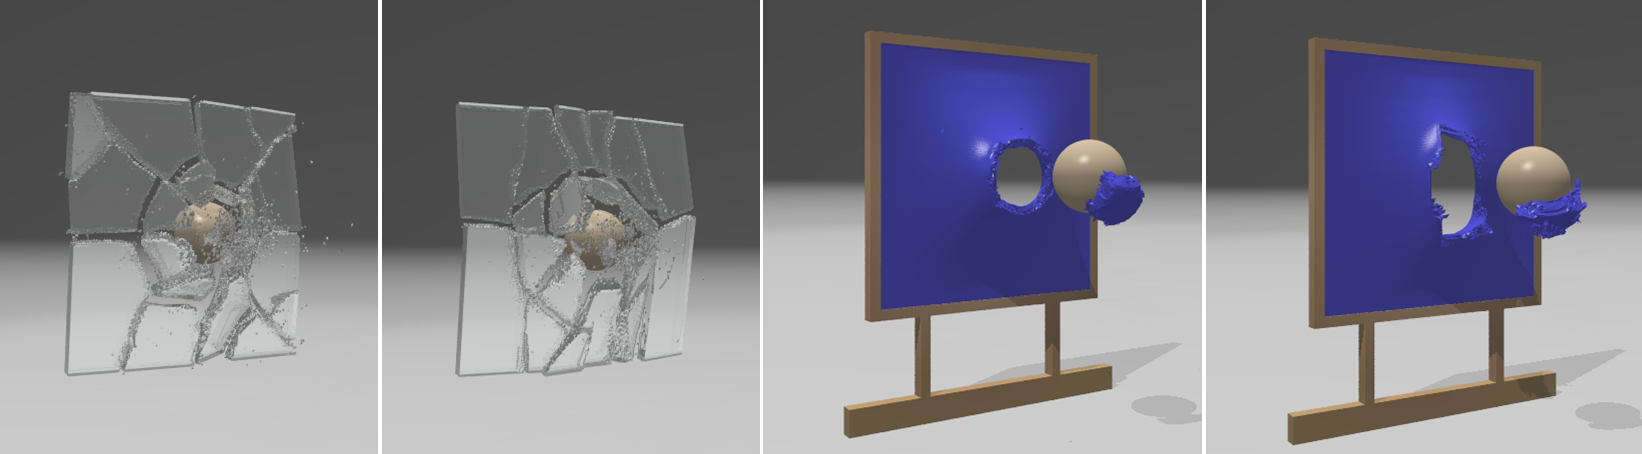
\includegraphics[width=\linewidth]{./figs/demo_impact.png}
 \centering
  \caption{ A sphere shoots through walls made of different materials, causing varied fracture behaviors. From left to right: isotropic brittle fracture, anisotropic brittle fracture, isotropic ductile fracture, anisotropic ductile fracture.}
\label{fig:1}
}

\maketitle

\begin{abstract}
In this paper, we exploit the use of peridynamics theory for graphical animation of material deformation and fracture. We present a new meshless framework for elastoplastic constitutive modeling that contrasts with previous approaches in graphics. Our peridynamics-based elastoplasticity model represents deformation behaviors of materials with high realism. We validate the model by varying the material properties and performing comparisons with FEM simulations. Besides, the integral-based nature of peridynamics makes it trivial to model material discontinuities, which outweighs differential-based methods in both accuracy and ease of implementation. We propose a simple strategy to model fracture in the setting of peridynamics discretization. We demonstrate that the fracture criterion combined with our elastoplasticity model could realistically produce ductile fracture as well as brittle fracture. Our work is the first application of peridynamics in graphics that could create a wide range of material phenomena including elasticity, plasticity, and fracture. The complete framework provides an attractive alternative to existing methods for producing modern visual effects.

\begin{classification} % according to http://www.acm.org/class/1998/
\CCScat{Computer Graphics}{I.3.7}{Three-Dimensional Graphics and Realism}{Animation}
\end{classification}

\end{abstract}

%-------------------------------------------------------------------------
\section{Introduction}

The simulation of deformable materials has been an important research topic in computer graphics for decades, since the early work by Terzopoulos and colleagues \cite{Terzopoulos:1987:EDM:37402.37427}. One of the strongest driving forces behind the active research is the persistently growing needs for higher realism from the visual effects industry. Materials in real-world exhibit complex behaviors, such as coupled elastoplastic deformations, fracture, etc. The complicated material behaviors are difficult to be virtually replicated by any single method despite the numerous ones that have been developed thus far. Existing approaches generally excel at some phenomena but would stumble (if not fail) at others. For instance, mesh-based methods \cite{Muller:2004:IVM:1006058.1006087,Irving:2004:IFE:1028523.1028541,Teran:2005:RQF:1073368.1073394,Sifakis:2012:FSD:2343483.2343501} are a good choice to simulate elastic deformations whereas not preferred for phenomena that involve topological changes. Particle-based methods \cite{Muller:2003:PFS:846276.846298,Pauly:2005:MAF:1073204.1073296,Stomakhin:2013:MPM:2461912.2461948} are considered suitable for modeling topological changes, however the inherent loss of connectivity information would cause undesirable numerical fracture \cite{Liu:2011:AKM:2065362.2066108, Zhu:2016MPM} while simulating large deformations.

We build on recent developments of peridynamics theory in the computational physics community \cite{Silling2000,silling2007peridynamic,mitchell2011nonlocal, emmrich2013peridynamics,madenci2014peridynamic} and propose a novel framework for graphical animation of varied deformation behaviors and fracture. Our aim is to enrich available options of simulation techniques for easier and better animation production. Peridynamics was first adopted to animation applications by Levine et al. \cite{Levine:2015:PPS:2849517.2849526}. They described a simple spring-mass system to handle brittle fracture of solids. In contrast, we handle elastoplasticiy, brittle fracture, and ductile fracture in a single framework. To this end, we propose several novel contributions in this work. We first present an elastoplastic constitutive model in the peridynamics-based framework with simple extension to anisotropy, and the model is validated against results produced by FEM. Furthermore, we show that both brittle and ductile fracture phenomena can be naturally represented with nearly no effort by integrating a simple fracture criterion into this material model. This is due to the integral-based formulation of peridynamics, in which forces at a material point are computed by gathering contributions from all material points in its interaction range through integration. On the other hand, methods based on classical continuum mechanics formulate force computations with partial differential equations that fail to be applicable directly on singularities such as a crack. This feature makes our peridynamics-based framework more attractive over existing approaches for producing animations that involve fracture. Lastly, our method is simple to implement and trivially parallelizable, providing a useful alternative to previous methods for animation production.

%-------------------------------------------------------------------------
\section{Related Work}

A large body of literature has been devoted to physical simulation of natural phenomena as a result of active research. A complete literature review is beyond the scope of this paper. In the following we comment only on the representative works most related to ours.

\noindent{\textbf{Elastoplasticity Animation}}~The modeling of deformable plasticity in graphics dates back to the pioneering work by Terzopoulos and Fleischer \cite{Terzopoulos:1988:MID:378456.378522}. O'Brien and colleagues \cite{O'Brien:2002:GMA:566654.566579} incorporated a similar additive plasticity model into a finite element simulation to animate ductile fracture. The strain measure was decomposed into two components, where one is due to elastic deformation and the other due to plastic deformation. M\"{u}ller et al. \cite{Muller:2004:PBA:1028523.1028542} applied this model in their point-based animation framework and simulated plastic behaviors of objects.  Irving et al. \cite{Irving:2004:IFE:1028523.1028541} presented a multiplicative formulation of plasticity and pointed out that their model was better handling finite plastic deformation than the additive one. In contrast to the additive model, they decomposed the deformation gradient into two components through multiplication. The multiplicative model was extensively used by later works to animate phenomena that involve plasticity. Bargteil et al. simulated large viscoplastic flow\cite{Bargteil:2007:FEM:1276377.1276397}, Gerszewski and his colleagues animated elastoplastic solids\cite{Gerszewski:2009:PMA:1599470.1599488}, and Stomakhin et al. modeled plasticity of snow\cite{Stomakhin:2013:MPM:2461912.2461948}, just to name a few. Unfortunately, neither of the above plasticity models applies in the peridynamics framework because there is no concept of strain nor deformation gradient in the integral-based formulation. As a result, we present a new constitutive model for peridynamics in this work to animate elastoplastic solids.

\noindent{\textbf{Fracture Animation}}~Numerous methods have been proposed on fracture animation \cite{muguercia2014fracture,Wu:2015:SPB:2858852.2858866} because the stunning phenomenon of fracture and failure is an indispensable visual element in animated movies and video games. Early approaches use simple schemes to model fracture, such as the finite difference method \cite{Terzopoulos:1988:MID:378456.378522}, the mass-spring system \cite{Norton:1991:AFP:115244.115248}, and the mass-point constraint system\cite{smith2001fast}. O'Brien and colleagues \cite{O'Brien:1999:GMA:311535.311550} adopted techniques from continuum mechanics and presented a FEM-based method to simulate brittle fracture of solids. They later extended their method to ductile fracture by incorporating a plasticity model\cite{O'Brien:2002:GMA:566654.566579}. M\"{u}ller et al. \cite{Muller2001} employed a quasi-static finite element analysis to animate brittle fracture of stiff materials undergoing collisions. Parker et al. \cite{Parker:2009:RDF:1599470.1599492} presented some useful techniques for real-time simulation of fracture in game environment. One major issue in FEM-based methods is the generation of fracture patterns on meshes, which could alter the underlying mesh topology. Early methods typically made use of simple separation along mesh element boundaries \cite{Norton:1991:AFP:115244.115248,Mazarak:1999:AEO:351631.351688,smith2001fast,Muller2001} or even element deletion \cite{forest2002removing}. Mesh subdivision prior to splitting could somewhat increase the available geometric details \cite{Mor:2000:MST:646923.710372,Bielser:2000:ISS:826029.826523}, whereas this tended to introduce elements with poor aspect ratios. Allowing failure along more arbitrary paths could generate more geometrically rich fracture patterns \cite{Neff:1999:VMB:351631.351686,O'Brien:1999:GMA:311535.311550,O'Brien:2002:GMA:566654.566579}, albeit with the expense of complicated re-meshing. Molino et al. \cite{Molino2004} proposed a virtual node algorithm to avoid the complexity of re-meshing, where elements were duplicated into partially filled counterparts with virtual nodes. The virtual node algorithm was frequently used by subsequent works on fracture animation \cite{Bao:2007:FRM:1263129.1263275} and mesh cutting \cite{Sifakis:2007:ACD:1272690.1272701,Wang:2015:AVN:2849517.2849531} due to its simplicity compared to re-meshing methods. Other representative mesh-based methods resorted to modal analysis \cite{glondu2013real} and pure geometric mesh decompositions \cite{Muller:2013:RTD:2461912.2461934,Schvartzman:2014:FAB:2556700.2556713} for real-time brittle fracture. Most recently, several works explored the boundary element method for rigid body fracture \cite{Zhu:2015:SRB:2809654.2766942,Hahn:2015:HBF:2809654.2766896} where only surface meshes were employed for both representation and computation.

In contrast to mesh-based approaches, meshless methods are generally considered as a better solution for animating topological changes. Based on the moving least square (MLS) meshless framework by M\"{u}ller et al. \cite{Muller:2004:PBA:1028523.1028542}, Pauly and colleagues \cite{Pauly:2005:MAF:1073204.1073296} developed a novel meshless method for fracture animation of elastoplastic solids. Steinemann et al. \cite{Steinemann:2009:SMD:1651926.1652002} employed surface mesh representation in meshless framework and presented a novel surface tracking technique to efficiently split the meshless deforming objects. Inspired by the rigid body assumption for simulating brittle fracture, Liu et al. \cite{Liu:2011:MSB:1970281.1970303} employed quasi-static analysis in a meshless local Petrov-Galerkin framework. Stomakhin et al. modeled the fracture of snow using a meshless material point method \cite{Stomakhin:2013:MPM:2461912.2461948}. Hegemann et al. \cite{Hegemann:2013:LSM:2485895.2485908} combined a level set based mesh embedding technique with the material point method to animate dynamic ductile fracture.

\noindent{\textbf{Peridynamics}}~The peridynamics theory was first proposed by Silling \cite{Silling2000} as a nonlocal reformulation of classical solid mechanics. It contrasts with classical (local) theory in that the state of a material point is influenced by not necessarily the material points located in its immediate vicinity, but also those over long distances. The governing equations of the peridynamics theory are spatial integral equations instead of partial differential equations. The theory was further developed by subsequent works \cite{silling2007peridynamic,emmrich2013peridynamics}, and its applications to the engineering field such as multi-scale material modeling \cite{askari2008peridynamics,silling2014hierarchical} and fracture modeling \cite{askari2006peridynamic,silling2010crack,silling2014peridynamic} were studied. A comprehensive review of the research literature in the computational physics community is beyond our scope, we refer the readers to the book by Madenci and Oterkus \cite{madenci2014peridynamic}.  Levine et al. \cite{Levine:2015:PPS:2849517.2849526} first introduced peridynamics to graphics for fracture animation. Their method was limited to brittle fracture of isotropic elastic materials with a single Poisson ratio of 0.25. Our work, on the other hand, is a complete framework that models elastoplasticity and anisotropy under various parameter settings, representing brittle and ductile fracture with high realism.

%-------------------------------------------------------------------------
\section{Background}\label{section:3}

The peridynamics theory models a continuum with particles, where any particle $\mathbf{x}$ interacts with other particles within a distance $\delta$. The distance $\delta$ is called the \textbf{horizon} of $\mathbf{x}$, and the particles within the horizon are referred as its \textbf{family}, $H_\mathbf{x}$. See Figure~\ref{fig:2} for an illustration of the peridynamics discretization. It seems analogous to other meshless methods based on classical theory \cite{Muller:2003:PFS:846276.846298,Muller:2004:PBA:1028523.1028542}, and the difference lies in the scale of interaction radius $\delta$. In the case of the classical (local) continuum model, the state of a particle is influenced by only particles in its immediate vicinity. In the case of the peridynamics theory, however, the state of a particle is influenced by particles within a region of finite radius. The peridynamics theory is thus referred as a nonlocal theory. As the radius becomes infinitely large, the peridynamics theory becomes the continuous version of the molecular dynamics model. As the radius becomes smaller, it becomes the continuum mechanics model. Therefore, the peridynamics model establishes a connection between the continuum mechanics and molecular dynamics models.

Our motivation for choosing peridynamics is that it is better able to handle material discontinuities, such as cracks. This is due to its formulation of governing equations as spatial integral equations, which stands in contrast to the partial differential equations used in the classical formulations. As we know, spatial derivatives are not well defined at discontinuities. Therefore, special treatment is generally required for fracture modeling in existing methods that are based on classical continuum mechanics. For instance, the mesh-based methods \cite{O'Brien:1999:GMA:311535.311550,O'Brien:2002:GMA:566654.566579} employed re-meshing operations and the meshless method by Pauly et al. \cite{Pauly:2005:MAF:1073204.1073296} altered the particle weight functions. The peridynamics governing equations are well defined at discontinuities, and material damage is represented as part of the peridynamics constitutive model. These attributes permit fracture initiation and propagation to be modeled with arbitrary paths in the peridynamics framework.

In peridynamics, the governing equation at any point $\mathbf{x}$ is \nobreak{formulated} as below:
\begin{equation}
\rho\ddot{\mathbf{u}}(\mathbf{x}) = \int_{H_\mathbf{x}}[\mathbf{T}<\mathbf{x}'-\mathbf{x}> - \mathbf{T}<\mathbf{x}-\mathbf{x}'>]dV_{\mathbf{x}}+\mathbf{b}(\mathbf{x}),
\label{eq:1}
\end{equation}
where $\rho$ is the mass density, $\mathbf{u}$ denotes the displacement, $\mathbf{b}$ is the external loads due to gravity and impact forces, $V_\mathbf{x}$ is the volume of $\mathbf{x}$, and $\mathbf{x}'$ is one material point that belongs to the family $H_{\mathbf{x}}$ of $\mathbf{x}$. $\mathbf{T}<\mathbf{x}'-\mathbf{x}>$ and $\mathbf{T}<\mathbf{x}-\mathbf{x}'>$ are two essential terms in which the constitutive laws of materials are encoded. $\mathbf{T}<\mathbf{x}'-\mathbf{x}>$ represents the internal force density that is exerted on $\mathbf{x}$ by $\mathbf{x}'$, and $\mathbf{T}<\mathbf{x}-\mathbf{x}'>$ is the other way around. The two terms both appear in the governing equation to enforce the Newton's third law, and similar strategy was employed in SPH methods\cite{Muller:2003:PFS:846276.846298}. The angle brackets representation $<\cdot>$ was defined by Silling et al. \cite{silling2007peridynamic} as a function inside the family $H_\mathbf{x}$, which they called as a \textbf{state}. Please note the integral form of the equation, which is the key difference between peridynamics and classical theory. The entire framework is built on displacements $\mathbf{u}$ instead of their spatial derivatives, thereby making discontinuity modeling trivial.

\begin{figure}[t]
  \centering
  %\mbox{} \hfill
  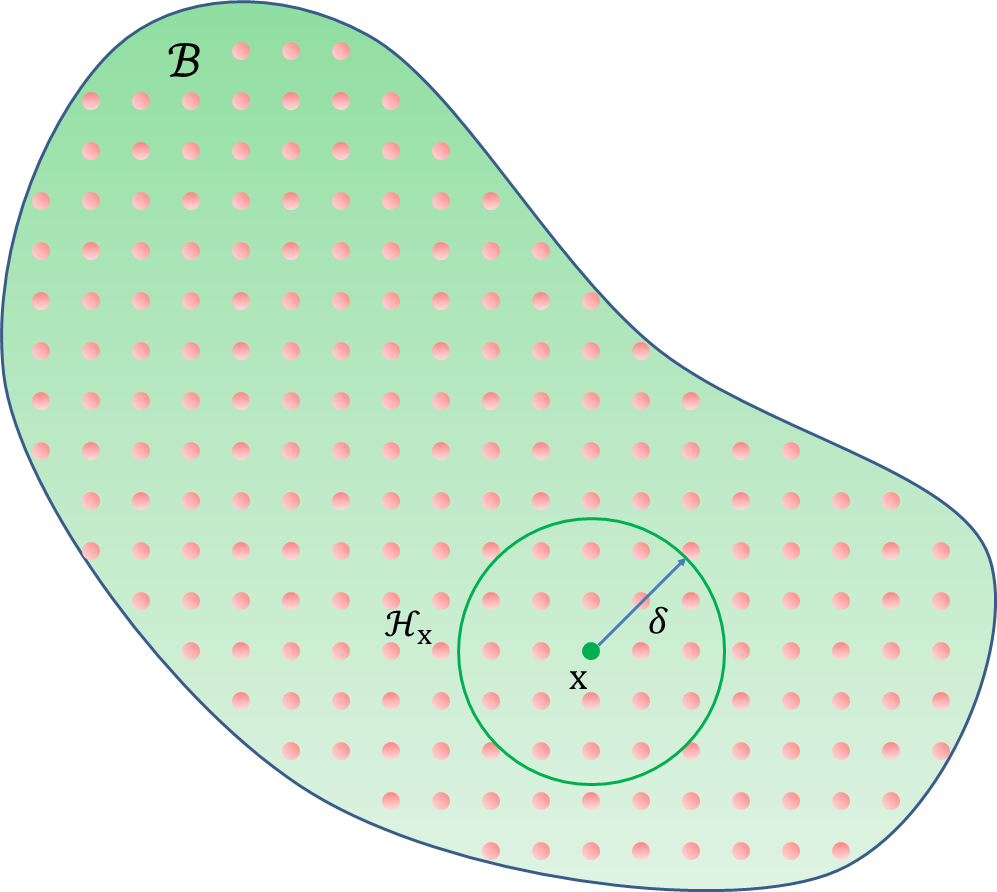
\includegraphics[width=0.7\linewidth]{./figs/peridynamics_circle.png}
  \caption{\label{fig:2}
  Illustration of peridynamics discretization. A continuum is represented as particles (pink dots), and any particle (green dot) interacts with the particles within its horizon (green circle).
}
\end{figure}

%-------------------------------------------------------------------------
\section{Elastoplastic Model}

In this section we describe our constitutive model for peridynamics in detail. We start with the basic isotropic elastic model, then plasticity is incorporated, and finally we extend the model with anisotropy.

\subsection{Isotropic Elasticity}\label{section:4.1}

As is discussed in Section~\ref{section:3}, the key to peridynamics-based constitutive modeling is the design of proper internal force density $\nobreak{\mathbf{T}<\cdot>}$. Silling et al.\cite{silling2007peridynamic} showed that peridynamic constitutive models can be designed to match many hyperelastic constitutive models under the classical elasticity theory. We derive our model based on the model described by Madenci and Oterkus \cite{madenci2014peridynamic}, which matches the isotropic linear elasticity model in classical theory. The elastic internal force density exerted by particle $j$ on particle $i$ is defined as below:
\begin{equation}
\mathbf{T}_i<\mathbf{x}_j-\mathbf{x}_i> = \frac{1}{2}A\frac{\mathbf{y}_j-\mathbf{y}_i}{|\mathbf{y}_j-\mathbf{y}_i|},
\label{eq:2}
\end{equation}
where $\mathbf{x}$ and $\mathbf{y}$ denote the positions of particles before and after deformation respectively. The direction of the force density is along the deformed bond between the particles given by $\frac{\mathbf{y}_j-\mathbf{y}_i}{|\mathbf{y}_j-\mathbf{y}_i|}$. $A$ is a scalar that represents the force magnitude, and it is composed of two terms by addition $A = A_{dilation} + A_{distortion}$, namely the dilation term $A_{dilation}$ and the distortion term $A_{distortion}$.

The dilation term $A_{dilation}$ is due to the dilation part of \nobreak{deformation}, i.e., volume change without any shape distortion. It is defined as:
\begin{equation}
A_{dilation}=4\omega_{ij}d\frac{\mathbf{y}_j-\mathbf{y}_i}{|\mathbf{y}_j-\mathbf{y}_i|}\cdot\frac{\mathbf{x}_j-\mathbf{x}_i}{|\mathbf{x}_j-\mathbf{x}_i|}a\theta_i.
\label{eq:3}
\end{equation}
$d$ and $a$ are both peridynamics material parameters, and $\omega_{ij}$ is the weight function between particle $i$ and particle $j$. For isotropic materials $\omega_{ij}$ is monotonically decreasing with respect to the distance between particles:
\begin{equation}
\omega_{ij} = \frac{\delta}{|\mathbf{x}_j-\mathbf{x}_i|}.
\label{eq:4}
\end{equation}
Note that $\omega_{ij}$ is defined in the material space, therefore can be precomputed. $\theta_i$ measures the dilation at particle $i$ defined with respect to the stretch of all bonds between particle $i$ and its family:
\begin{equation}
\theta_i = d\sum_{k=1}^N\omega_{ik}s_{ik}\frac{\mathbf{y}_k-\mathbf{y}_i}{|\mathbf{y}_k-\mathbf{y}_i|}\cdot(\mathbf{x}_k-\mathbf{x}_i)V_k,
\label{eq:5}
\end{equation}
where $N$ represents the number of family points $k$ for point $i$, and $V_k$ are their volumes. The stretch $s_{ik}$ of the bond  between particles is defined as:
\begin{equation}
s_{ik}=\frac{|\mathbf{y}_k-\mathbf{y}_i|}{|\mathbf{x}_k-\mathbf{x}_i|} -1.
\label{eq:6}
\end{equation}

The distortion term $A_{distortion}$ is a result of distortion deformation between particle $i$ and $j$. It is simply defined with respect to the extension of the bond between the two particles as:
\begin{equation}
A_{distortion}=4\omega_{ij}b(|\mathbf{y}_j-\mathbf{y}_i|-|\mathbf{x}_j-\mathbf{x}_i|),
\label{eq:7}
\end{equation}
with $\omega_{ij}$ as the weight function and $b$ is the material parameter.

The model is equivalent to the isotropic linear elasticity model in classical theory, please refer to the book\cite{madenci2014peridynamic} for elaborated derivation. Here we directly provide the conversion between the material parameters in this model and those from continuum mechanics:
\begin{equation}
a = \frac{1}{2}(\kappa-\frac{5\mu}{3}) \qquad b = \frac{15\mu}{2\pi\delta^5} \qquad d=\frac{9}{4\pi\delta^4},
\label{eq:8}
\end{equation}
where $\kappa$ and $\mu$ denote the bulk modulus and the shear modulus respectively.

In Figure~\ref{fig:3} we demonstrate an example of the hyperelastic deformations animated with our model.

\begin{figure}[t]
  \centering
  %\mbox{} \hfill
  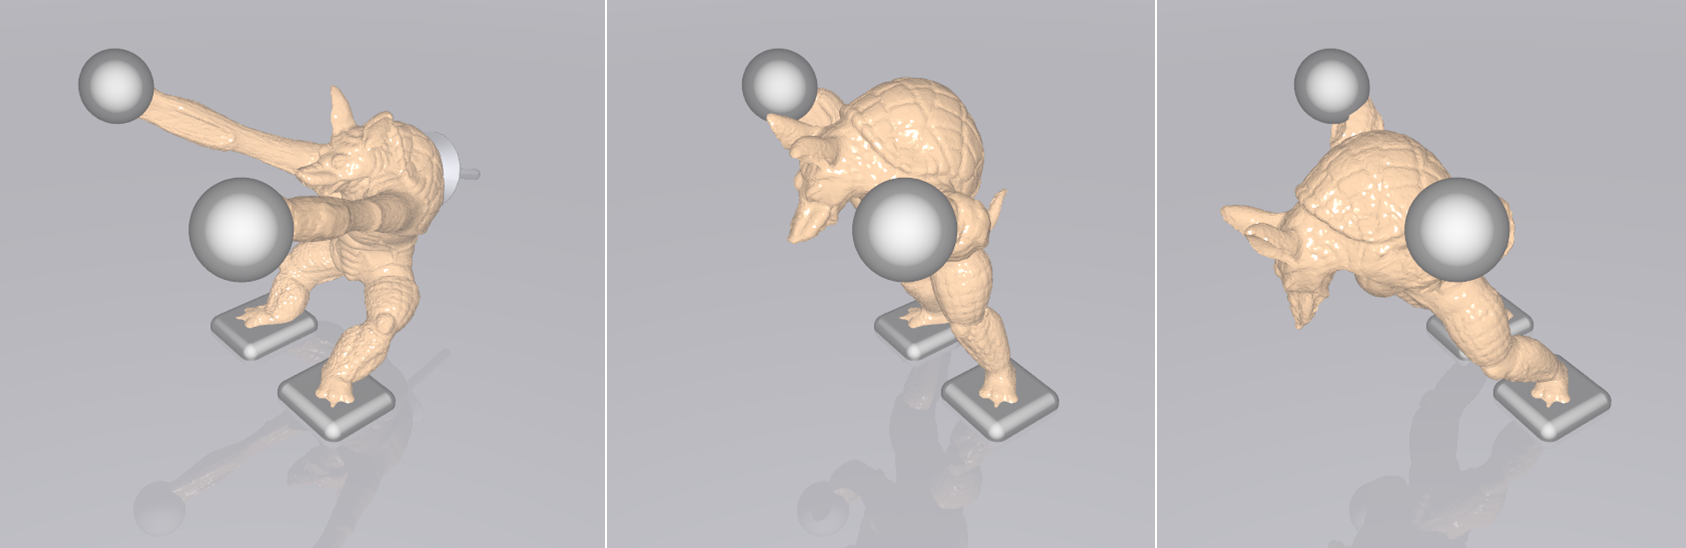
\includegraphics[width=\linewidth]{./figs/demo_pull_armadillo.png}
  \caption{\label{fig:3}
  Armadillo is initially anchored on its back and four limbs, and it deforms elastically when its back is released.
}
\end{figure}

\subsection{Plasticity}

Plasticity model for peridynamics is less studied in literature due to its complexity. To our knowledge, Silling et al. \cite{silling2007peridynamic} proposed the first plasticity model that is analogous to the von Mises flow model in classical theory. Mitchell presented a new framework for peridynamics-based plasticity modeling\cite{mitchell2011nonlocal} based on Silling et al.'s model, whereas the model hasn't been verified by experiments thus far. We adopt Mitchell's model for practical applications, and propose novel modifications based on their work.

Our plasticity model is based on purely deviatoric plastic flow theory, i.e., plastic flow takes place without change in volume. However, the dilation and distortion decomposition of our elasticity model (see Section~\ref{section:4.1}) can not fully sperate deviatoric deformations. Therefore, we perform some reformulation before introducing our plasticity model.

The reformulated elasticity model is additively composed by a deviatoric term $A_{deviatoric}$ and an isotropic term $A_{isotropic}$.

blabla

\begin{figure}[t]
  \centering
  %\mbox{} \hfill
  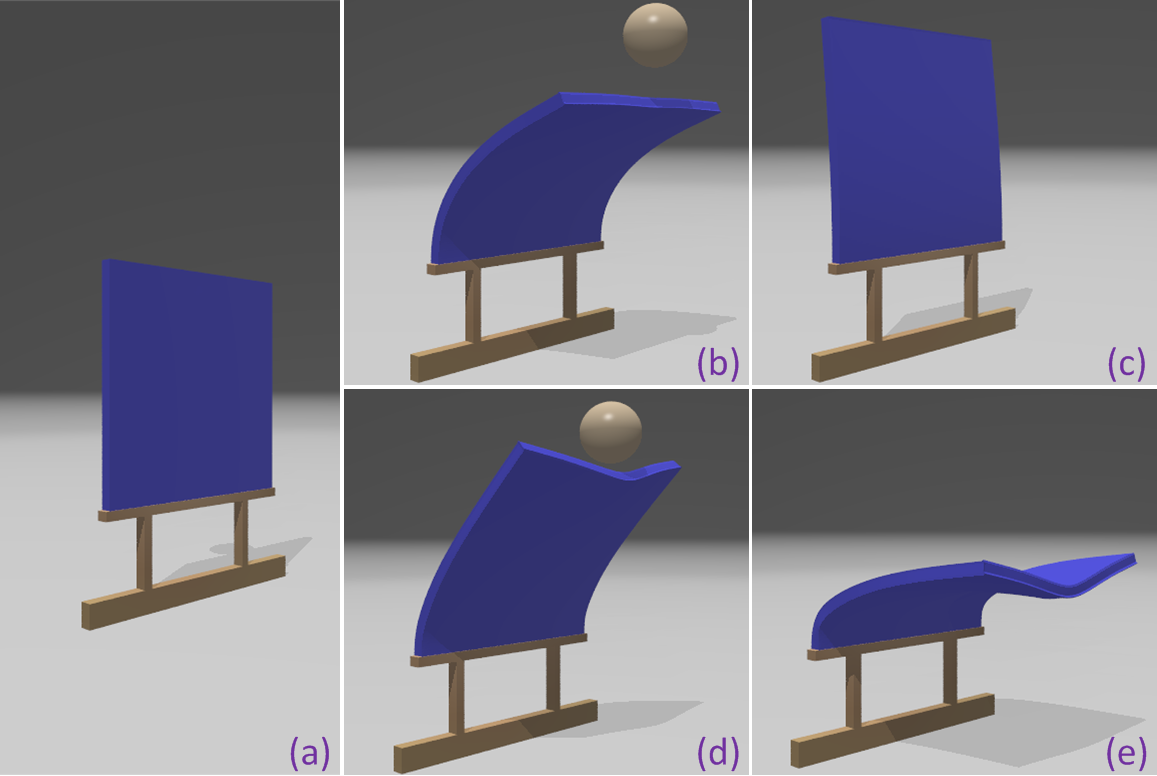
\includegraphics[width=\linewidth]{./figs/demo_impact_upside.png}
  \caption{\label{fig:4}
  Comparison of elastic and plastic deformations by shooting a sphere at two walls made of different materials with identical initial configuration as in (a). The elastic wall deforms on impact (b), and recovers afterwards (c). The plastic wall undergos permanent deformation (e) after the impact (d).
}
\end{figure}

\subsection{Anisotropy}

Our constitutive model is isotropic up to now, and we extend it to anisotropy in this section. We model anisotropy by manipulating the weight functions between particles (see Equation~\ref{eq:4}) with direction information. The key idea is to associate an anisotropy matrix $\mathbf{G}$ with each particle, so that applying the transformation to the bond between particles biases the influence weight toward preferred directions. Intuitively, the originally spherical shape of particle family (see Figure~\ref{fig:2}) is now an ellipsoid.

The weight function $\omega_{ij}$ for anisotropic materials is computed as below:
\begin{equation}
\omega_{ij}=\frac{\delta}{|\mathbf{G}(\mathbf{x}_j-\mathbf{x}_i)|}.
\end{equation}
Appealing anisotropic effects could be generated with our anisotropy model. See Figure~\ref{fig:1} for a demonstration of the model applied to brittle and ductile fracture animation. Figure~\ref{fig:5} compares the crack patterns generated by the brittle fracture examples in Figure~\ref{fig:1}.

\begin{figure}[t]
  \centering
  %\mbox{} \hfill
  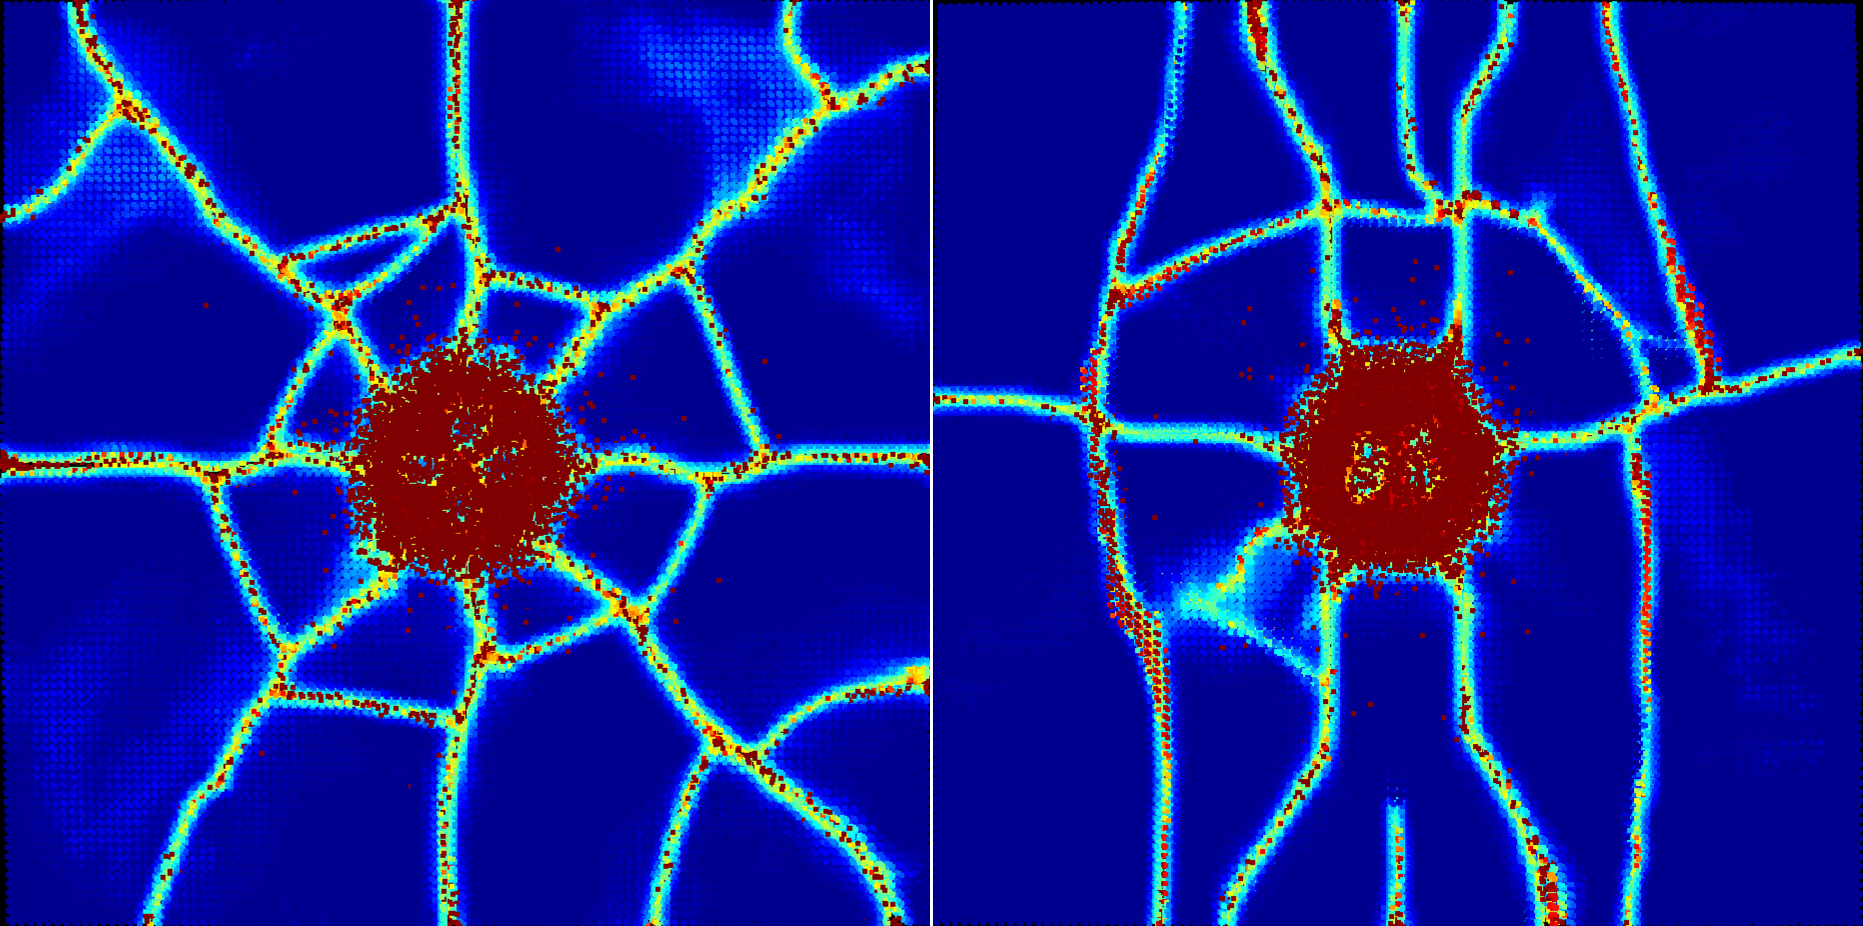
\includegraphics[width=\linewidth]{./figs/demo_impact_color_map.png}
  \caption{\label{fig:5}
  Comparison of crack patterns generated by isotropic (left) and anisotropic (right) brittle fracture. The color represents the damage of particles, with blue as no damage and red as complete damage.
}
\end{figure}

%-------------------------------------------------------------------------
\section{Fracture}

\emph{This section describes the fracture criterion, and the mesh split strategy. 0.5 page.}
\begin{figure*}[t]
  \centering
  %\mbox{} \hfill
  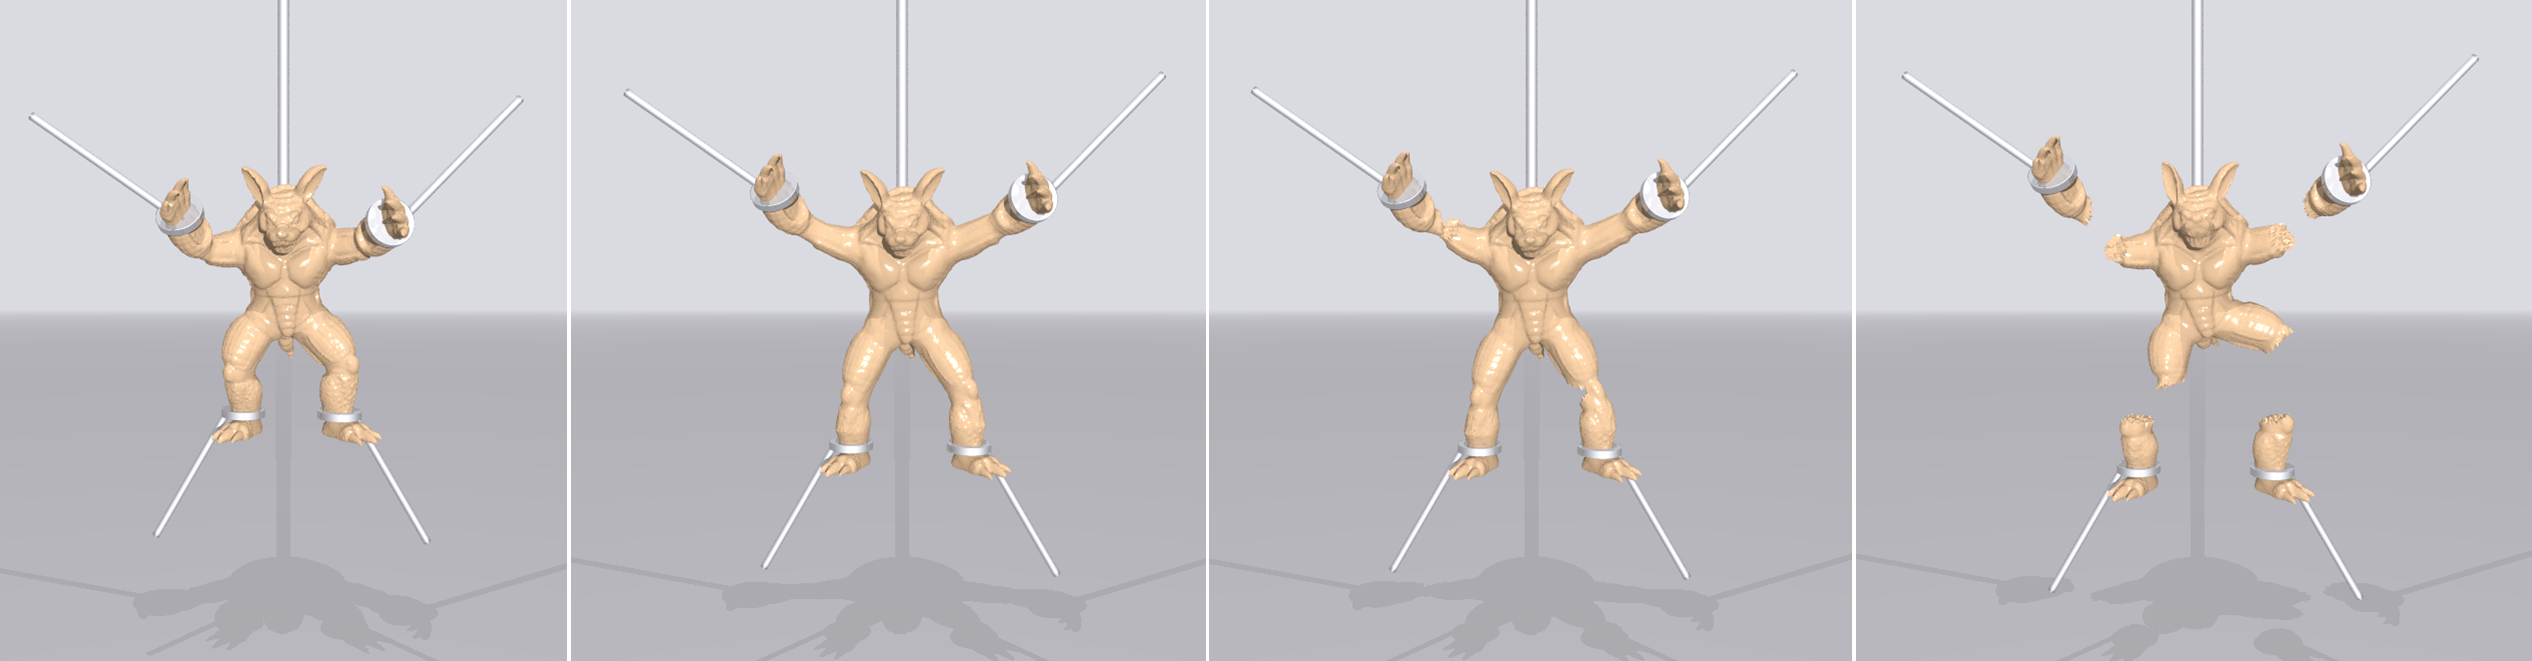
\includegraphics[width=\linewidth]{./figs/demo_tear_armadillo.png}
  \caption{\label{fig:6}
  tear armadillo figure.
}
\end{figure*}

\begin{figure}[h]
  \centering
  %\mbox{} \hfill
  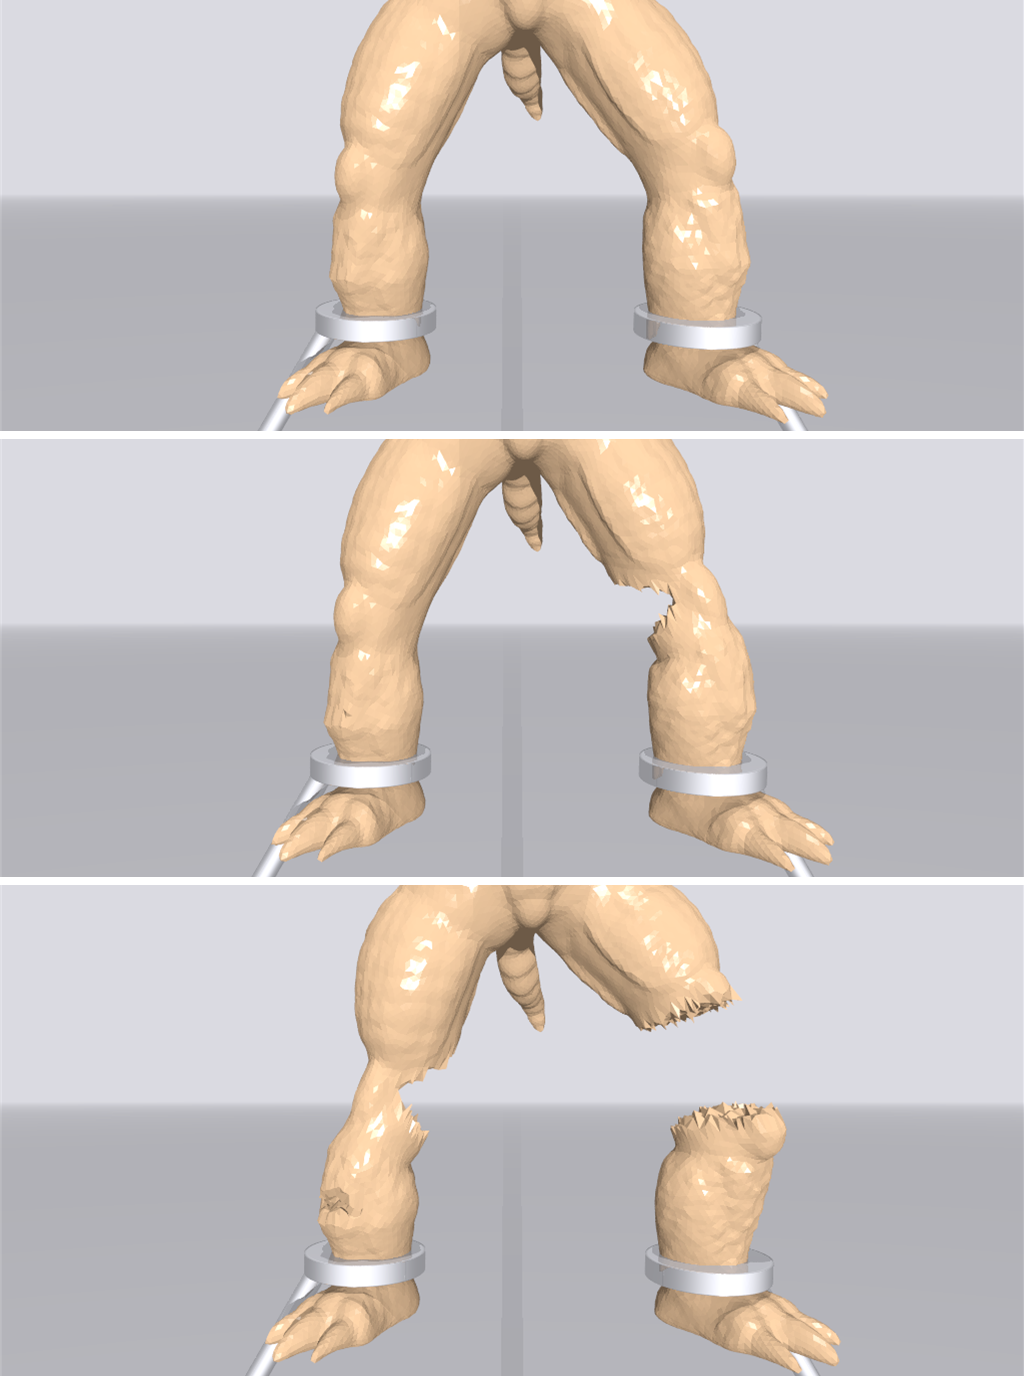
\includegraphics[width=\linewidth]{./figs/demo_tear_armadillo_close_view.png}
  \caption{\label{fig:7}
  tear armadillo close view.
}
\end{figure}

%-------------------------------------------------------------------------
\section{Results}

\emph{This section demonstrates some results. 1.5 page.}
\begin{figure}[h]
  \centering
  %\mbox{} \hfill
  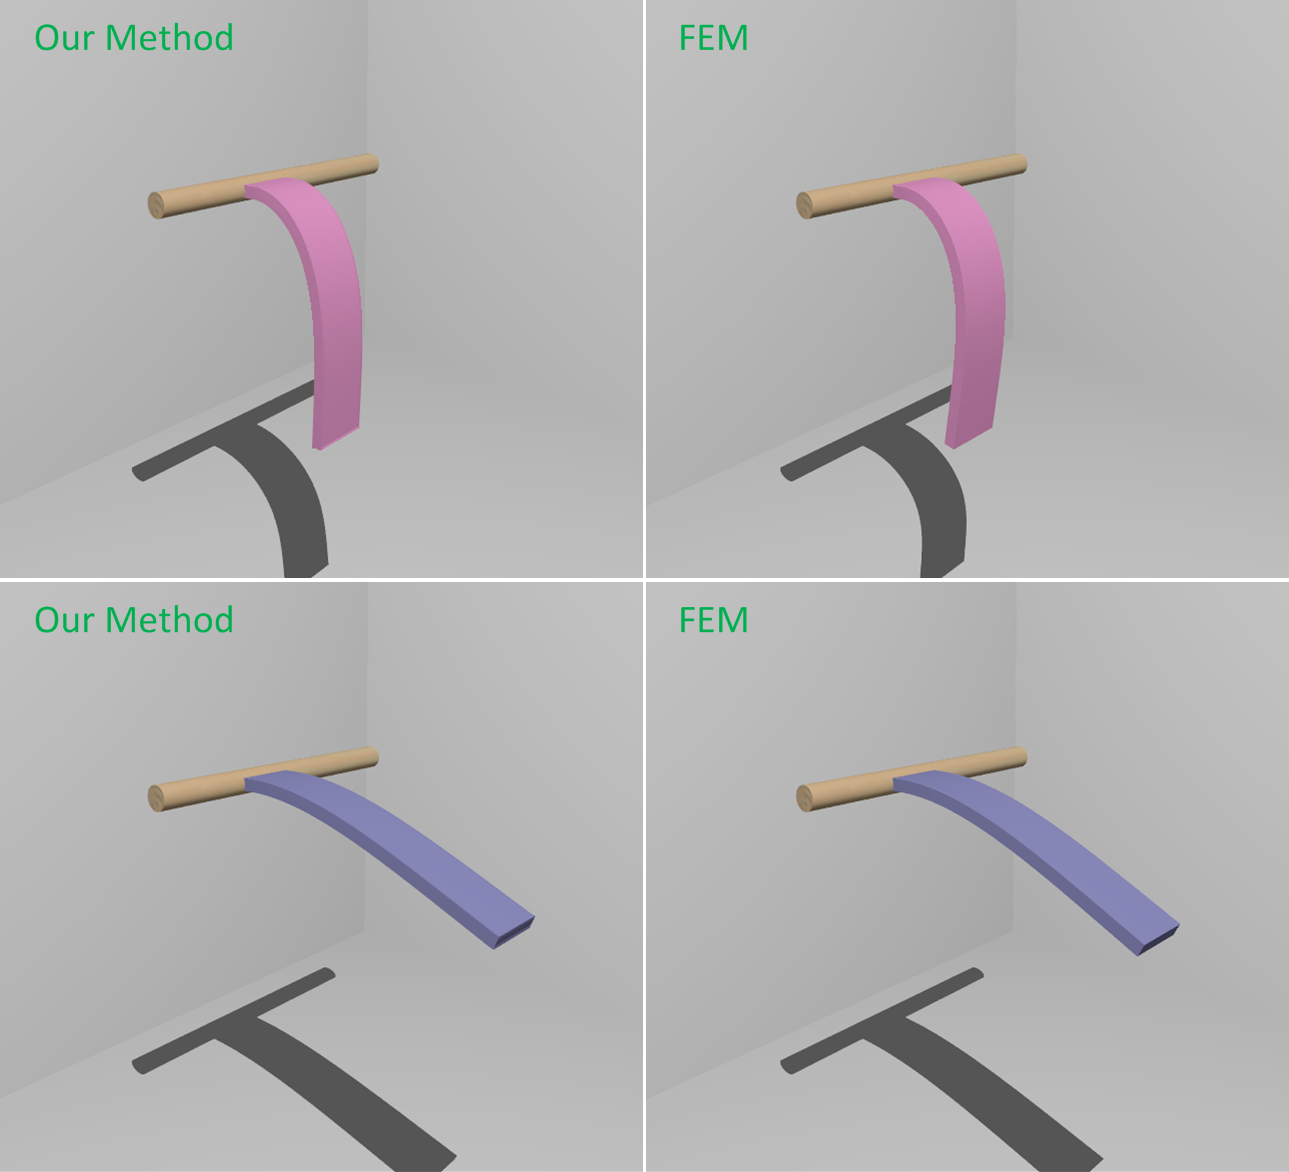
\includegraphics[width=\linewidth]{./figs/demo_strip_vs_fem.png}
  \caption{\label{fig:8}
  FEM validation.
}
\end{figure}
\begin{figure}[h]
  \centering
  %\mbox{} \hfill
  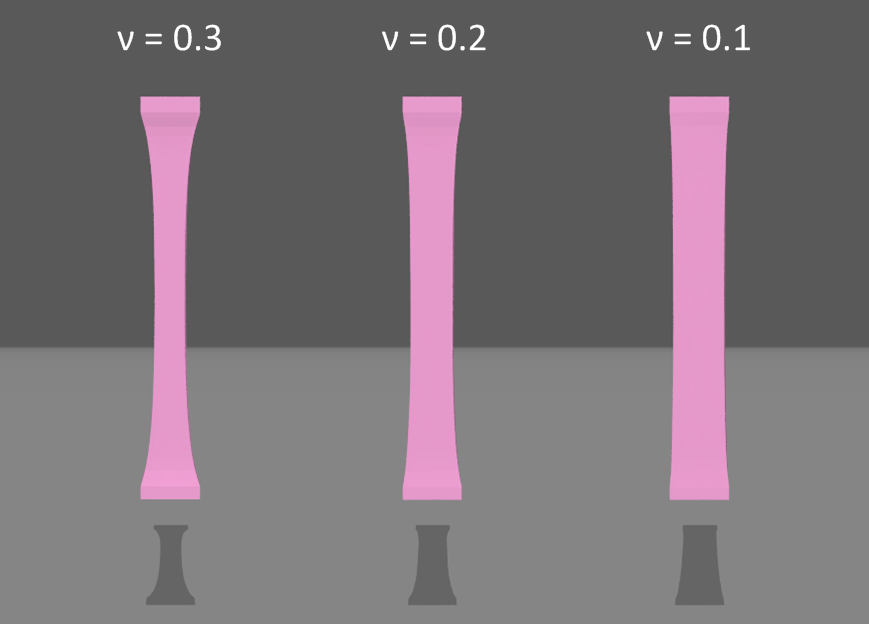
\includegraphics[width=\linewidth]{./figs/compare_different_poisson_ratio.png}
  \caption{\label{fig:9}
  poisson ratio.
}
\end{figure}
\begin{figure}[h]
  \centering
  %\mbox{} \hfill
  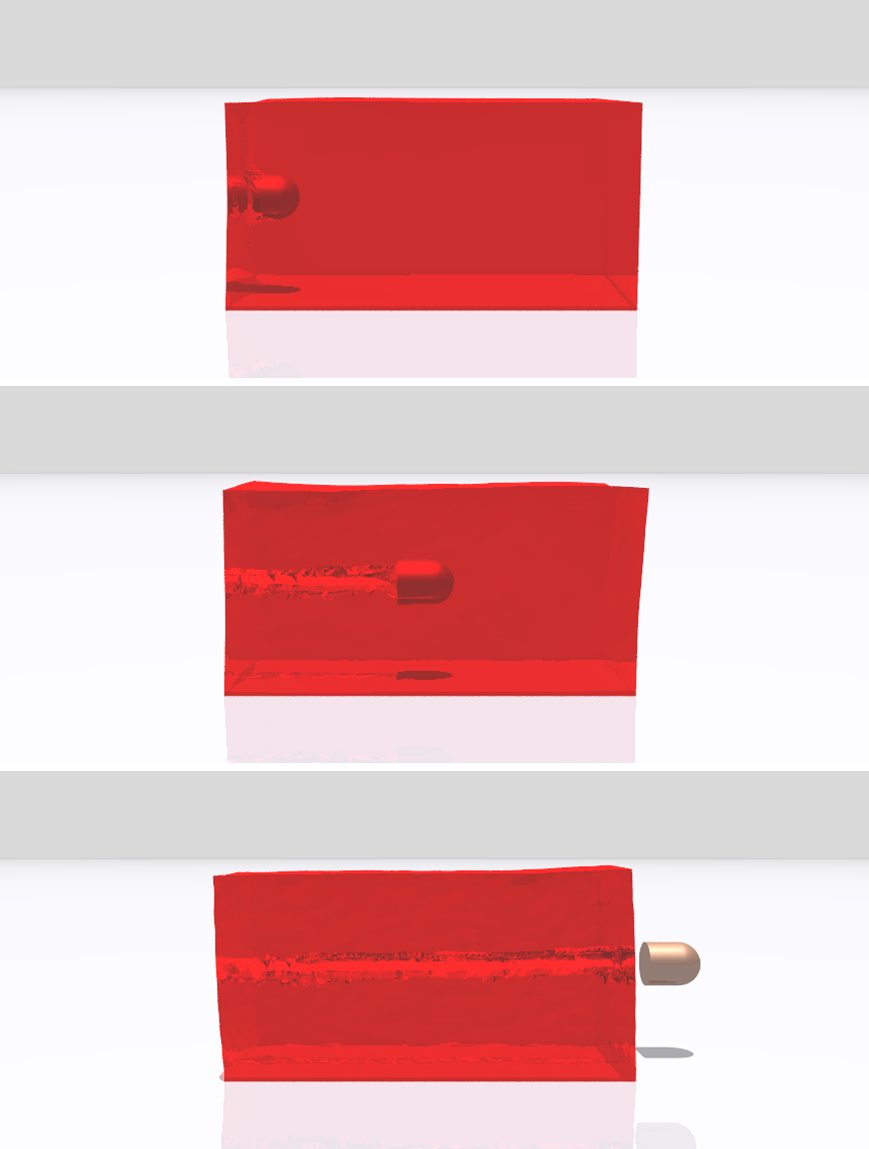
\includegraphics[width=\linewidth]{./figs/demo_jello.png}
  \caption{\label{fig:10}
  jello.
}
\end{figure}
\begin{figure*}[t]
  \centering
  %\mbox{} \hfill
  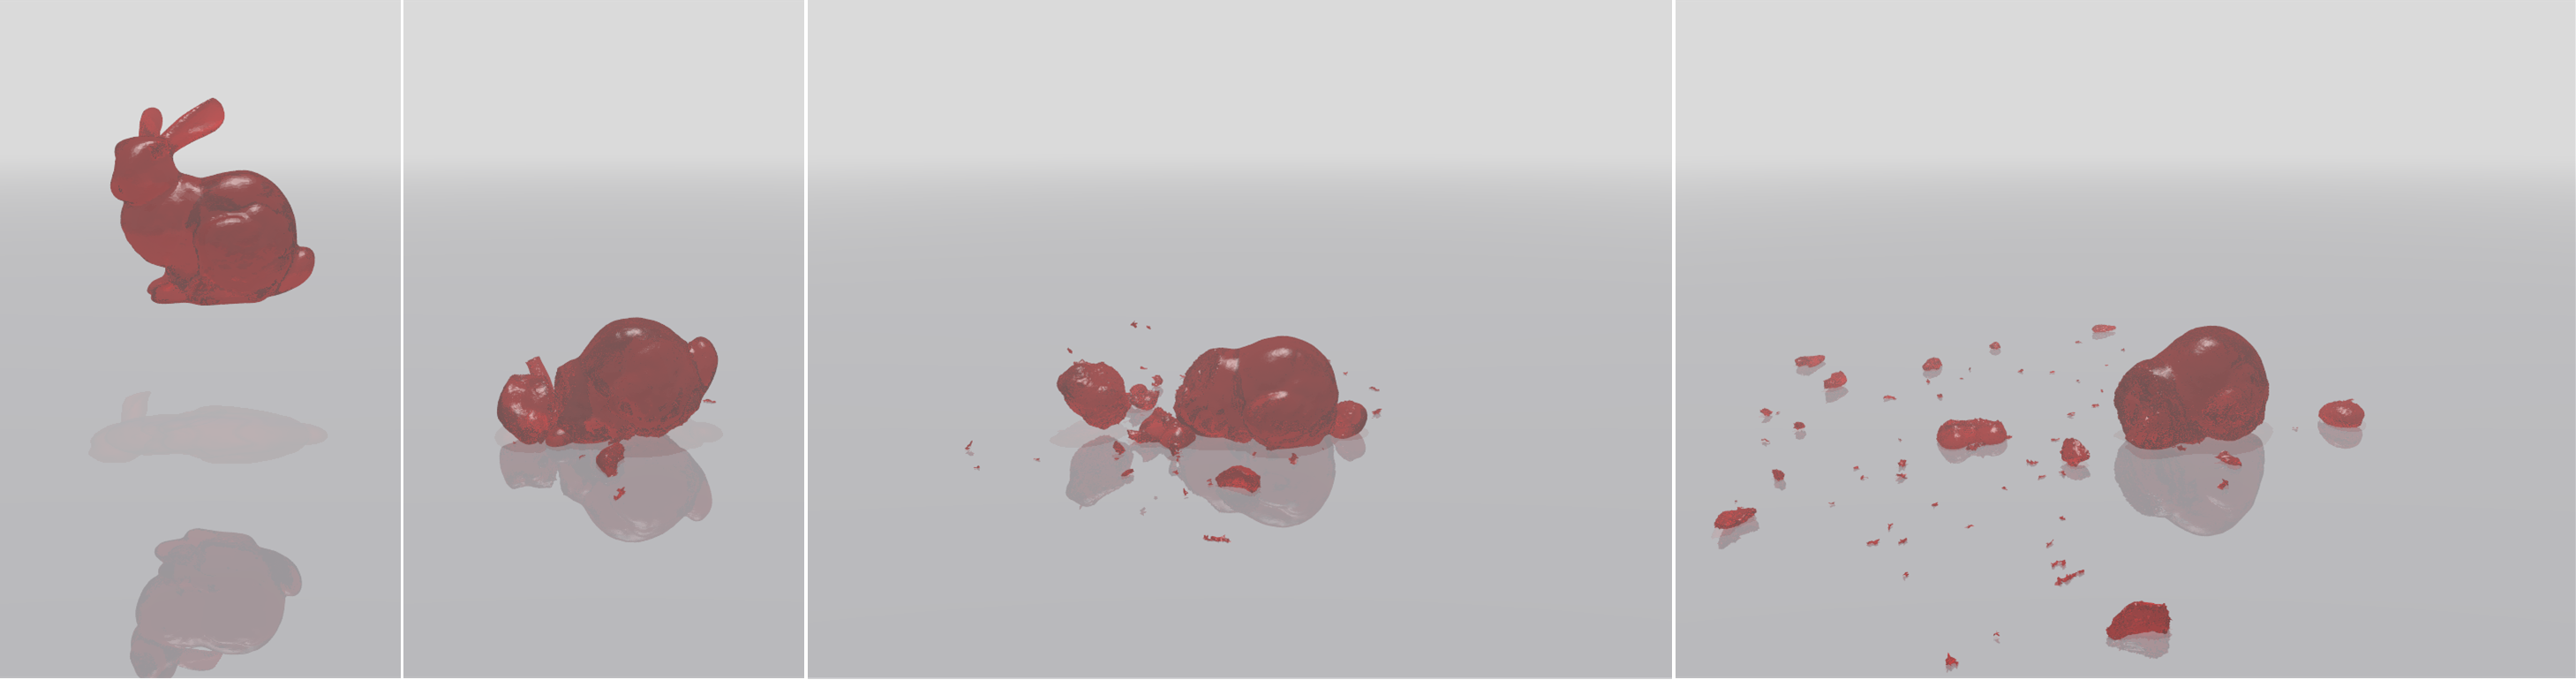
\includegraphics[width=\linewidth]{./figs/demo_fall_bunny.png}
  \caption{\label{fig:11}
  bunny fall.
}
\end{figure*}

\begin{figure}[h]
  \centering
  %\mbox{} \hfill
  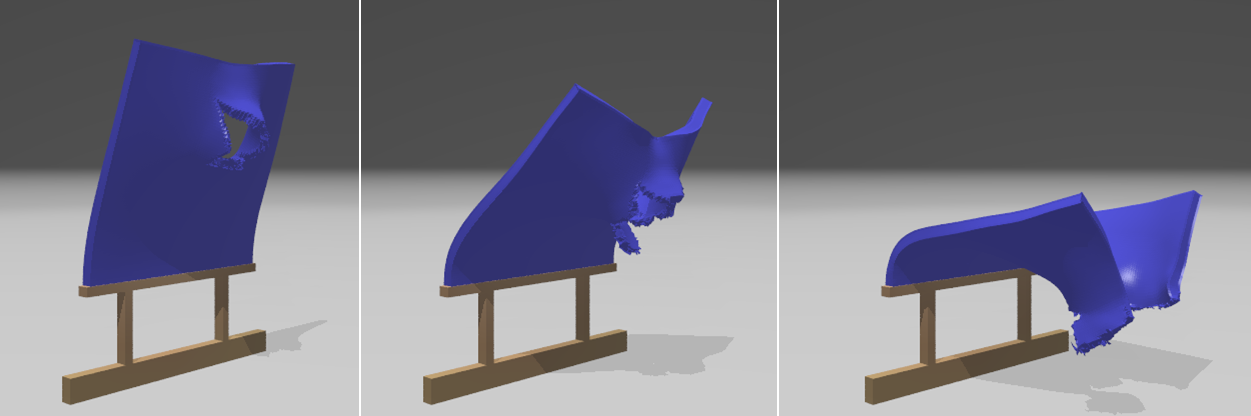
\includegraphics[width=\linewidth]{./figs/demo_impact_upside_plastic_fracture.png}
  \caption{\label{fig:12}
  up impact.
}
\end{figure}

%-------------------------------------------------------------------------
\section{Discussions}

\emph{This section concludes the paper, and discusses the limitations. 0.5 page.}

%-------------------------------------------------------------------------
\bibliographystyle{eg-alpha}
%\bibliographystyle{eg-alpha-doi}

\bibliography{references}

%-------------------------------------------------------------------------
%\newpage

\end{document}
